\section{Data formats}
\label{sec:dataformats}

In this section we describe how polynomials, lists, marked Gr\"obner
bases etc. are represented as ASCII character strings. These strings
will be input to the programs by typing or by redirecting the standard
input and be output by the program on the standard output which may be
the screen, a pipe or a file. Usually files are used for input. For
example,
\begin{verbatim}
gfan_bases < inputfile.txt > outputfile.txt
\end{verbatim}
will read its input from {\tt inputfile.txt} and write its output to
{\tt outputfile.txt}. The following is an example of how to use pipes
for computing a universal Gr\"obner basis of the input:
\begin{verbatim}
gfan_bases < inputfile.txt | gfan_polynomialsetunion > outputfile.txt
\end{verbatim}
In general spaces and newlines in the input are ignored, but for the
polyhedral formats described in Section~\ref{sec:format fan} and
Section~\ref{sec:format cone} the rules are different.

\subsection{Fields}
Two kinds of fields are supported:
\begin{itemize}
\item The field $\Q$ of rationals which is represented by the string ``\texttt{Q}''.
\item Fields of the form $\Z/p\Z$ where $p$ is a prime number. These
fields are represented by text strings ``\texttt{Z/pZ}'' where \texttt{p}  is the
prime number. For example ``\texttt{Z/3Z}'' or ``\texttt{Z/17Z}''. In Gfan the
prime number $p$ must be less than $32749$.
\end{itemize}
\subsection{Variables}
A variable is denoted by its name which is an string of
characters. The exact rules for which names are allowed have not been
decided on in this version of Gfan and therefore Gfan accepts most
names. However, white spaces, commas and ``\texttt{]}'' are not allowed
as characters in the name. Furthermore one should not choose variable
names such that one name is a starting substring of an other -- don't
choose names such as ``\texttt{x1}'' and ``\texttt{x}''
in the same polynomial ring.
\subsection{Polynomial rings}
A polynomial ring is represented first by a field and then by a list of
variable names.  The list begins with ``\texttt{[}'' and ends with
``\texttt{]}''. Names are separated by commas. The ordering of the
variables matters as this is also the ordering used for the entries of
for example weight vectors. Examples: ``\texttt{Z/2Z[a,b]}'' and ``\texttt{Q[x\_1,x\_2,y1,y2]}''.
\subsection{Polynomials}
%The variables in the polynomial ring are named {\tt a},...,{\tt
%z},{\tt A},...,{\tt Z}. The number of variables in the polynomial ring
%is specified implicitly. It depends on the variables used in the
%input. It is important to note that the first variable is always {\tt
%a}, meaning that if, for example, {\tt h} is used then all variables
%from {\tt a} to {\tt g} are also used and memory is allocated for
%these variables. Thus the program will require more memory and be much
%slower if the user uses a variable without using the previous ones. %
%compared to start the naming with {\tt a}.  If you already have a file
%where the variables have different names then have a look at
%Subsection \ref{applist:_substitute}.

Coefficients in the field are given as fractions. A coefficient equals
its numerator multiplied by the inverse of the denominator. The
numerator and denominator themselves are given by an integer in $\Z$
which is mapped to the field by the homomorphism sending $1\in\Z$ to
$1$ in the field. The '{\tt /}' character and the denominator can be
left out if the denominator is $1$. If a field with non-zero
characteristic was chosen one should be careful that the denominator
is not $0$.

Monomials are written in the following formats:
\begin{itemize}
\item
\texttt{a\symbol{94}4dc}
\item
\texttt{a4dc}
\item
\texttt{aaadac}
\end{itemize}
The monomial $1$ cannot be written without writing it as a term in the usual way ``\texttt{1}''.
Any other term is either a monomial or a coefficient and a monomial. A polynomial is a list of terms separated by {\tt +}. The {\tt +} may be left out if the numerator of the next monomial is negative.

That description did not cover every detail. Here is an example:
\begin{verbatim}
hello world - 3/8 a2+23abcge^4 +1
\end{verbatim}
In our usual notation we would write it like this: $dehl^{3}o^{2}rw+1+23abce^{4}g-{3\over 8}a^{2}$.
{\bf It is important to note that the first term written in a polynomial is distinguished from the other terms in the polynomial. This is useful when specifying marked Gr\"obner bases.}
\subsection{Lists}
A list begins with a '{\tt \{}' or a '{\tt (}', contains elements separated by '{\tt ,}' and is ended by a  '{\tt \}}' or a '{\tt )}'.
Different types of lists may be needed when specifying input for the various programs:
\begin{description}
\item[An integer vector] is a list of integers.
\item[A list of integer vectors] is a list of integer vectors. Such lists are used for example when specifying generators for subgroups of $S_n$.
\item[A polynomial list] (or a polynomial set) is a list of polynomials.
\item[A Gr\"obner basis]  is the list of polynomials in a Gr\"obner basis with the leading term of each listed polynomial being the initial term with respect to a term order for which this a Gr\"obner basis.
\item[A list of polynomial sets] is a list of polynomial sets. Often the polynomial sets are required to be Gr\"obner bases.
\item[An ideal] is written as a list of polynomials generating it.
\end{description}
For all other lists than integer vectors the characters '{\tt \{}' and '{\tt \}}' are used to start and end the list.

\subsection{Permutations}
When exploiting the symmetry of an ideal one needs to input permutations to the program. Each permutation is specified by a vector. The length of the vector should equal the number of elements being permuted - for example the number of variables in the polynomial ring.
The first element in the vector describes where the first element goes and so on. Of course we start indexing from $0$. The following vectors specify the identity, a transposition and a 3-cycle, respectively, on an ordered set of four elements:

\begin{itemize}
\item {\tt (0,1,2,3)}
\item {\tt (1,0,2,3)}
\item {\tt (0,3,1,2)}
\end{itemize}


\subsection{Polyhedral fans}
\label{sec:format fan}
\label{format:fan}
The output format for polyhedral fans is intended to be Polymake \cite{polymake} compatible. Polymake recently switched to an XML based format. Gfan will keep outputting data in the old text style by default as it is more convienient for the command line Gfan user. The option \texttt{--xml} switches output to being XML. In the Polymake world, the output objects will have type \texttt{SymmetricFan}. The new XML files cannot be read by Gfan at the moment, while the old non-XML format cannot be read by any version of Polymake. In the following we describe only the text (non-XML) format. For the XML format we refer to the Polymake documentation.

The text representation of a fan begins with the lines
\begin{verbatim}
_application fan
_version 2.2
_type SymmetricFan
\end{verbatim}
After this follows a list of properties. For example
\begin{verbatim}
LINEALITY_SPACE
0 0 0 0 0 1 1 1 1 1 1 1 1 1 1
0 0 0 0 1 0 0 0 1 0 0 1 0 1 1
0 0 0 1 0 0 0 1 0 0 1 0 1 0 1
0 0 1 0 0 0 1 0 0 1 0 0 1 1 0
0 1 0 0 0 0 -1 -1 -1 0 0 0 -1 -1 -1
1 0 0 0 0 0 0 0 0 -1 -1 -1 -1 -1 -1
\end{verbatim}
Each property has a name and must be assigned a value of a certain type. You can read more about the philosophy of the format in the Polymake documentation.

\begin{example}
\label{ex:polyformat}
The ideal $I=\langle ab-c,bc-a,ca-b\rangle$ has a cyclic symmetry.
If we run the commands
\begin{verbatim}
gfan --symmetry -e | gfan_topolyhedralfan --symmetry
\end{verbatim}
on the input
\begin{verbatim}
Q[a,b,c]
{ab-c,bc-a,ca-b}
{(1,2,0)}
\end{verbatim}
we get a polyhedral representation of the Gr\"obner fan of $I$:
\begin{verbatim}
_application PolyhedralFan
_version 2.2
_type PolyhedralFan

AMBIENT_DIM
3

DIM
3

LINEALITY_DIM
0

RAYS
1 1 0	# 0
1 0 1	# 1
0 1 1	# 2
0 1 0	# 3
1 0 0	# 4
0 0 1	# 5
2 1 1	# 6
1 1 2	# 7
1 2 1	# 8
1 1 1	# 9

N_RAYS
10

LINEALITY_SPACE

ORTH_LINEALITY_SPACE
0 0 1
0 1 0
1 0 0

F_VECTOR
1 10 18 9

CONES
{}	# New orbit	# Dimension 0
{0}	# New orbit	# Dimension 1
{1}
{2}
{3}	# New orbit
{4}
{5}
{6}	# New orbit
{7}
{8}
{9}	# New orbit
{0 3}	# New orbit	# Dimension 2
{1 4}
{2 5}
{0 4}	# New orbit
{1 5}
{2 3}
{6 9}	# New orbit
{7 9}
{8 9}
{0 6}	# New orbit
{1 7}
{2 8}
{0 8}	# New orbit
{1 6}
{2 7}
{3 8}	# New orbit
{4 6}
{5 7}
{0 3 8}	# New orbit	# Dimension 3
{1 4 6}
{2 5 7}
{0 4 6}	# New orbit
{1 5 7}
{2 3 8}
{0 6 8 9}	# New orbit
{1 6 7 9}
{2 7 8 9}

MAXIMAL_CONES
{0 3 8}	# New orbit	# Dimension 3
{1 4 6}
{2 5 7}
{0 4 6}	# New orbit
{1 5 7}
{2 3 8}
{0 6 8 9}	# New orbit
{1 6 7 9}
{2 7 8 9}

PURE
1
\end{verbatim}
The most important properties are ``RAYS'' and ``CONES''. A ray is given by a relative interior point and a cone is given by a list of indices of rays that will generate the cone.
We may compare this combinatorial data
to the drawing of the Gr\"obner fan given in
Figure~\ref{fig:polyformat}. Notice that this example is particularly
simple as the dimension of the homogeneity space of $I$ is $0$.
\end{example}
\begin{figure}
\begin{center}
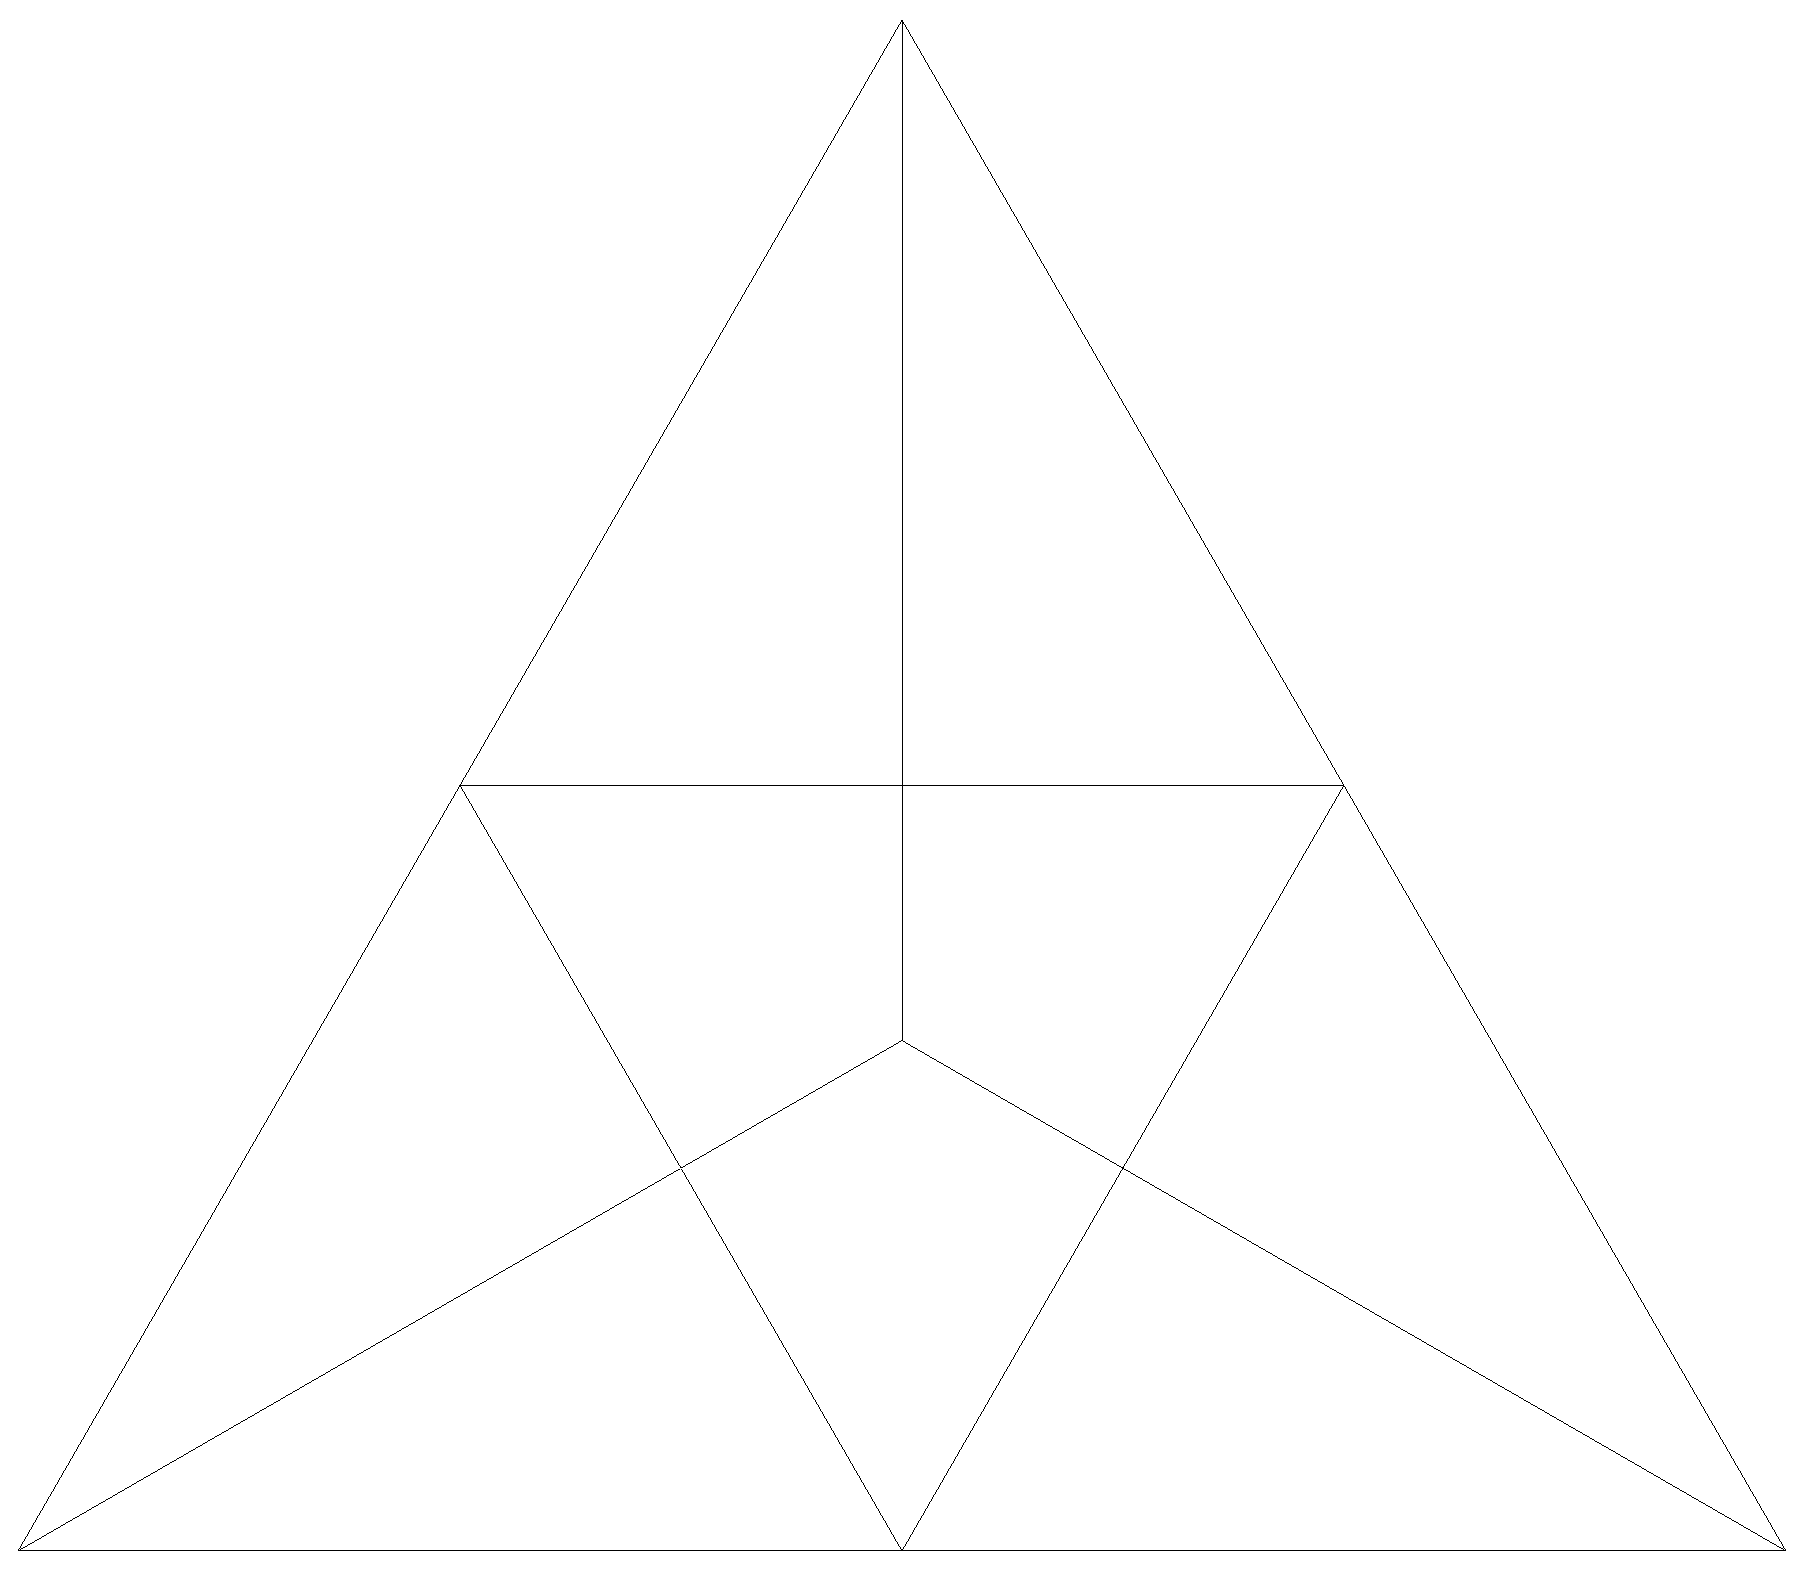
\epsfig{file=polyformat.eps,height=5.9cm} 
\end{center}
\caption{The Gr\"obner fan in Example~\ref{ex:polyformat} intersected with the standard simplex in $\R^3$.}
\label{fig:polyformat}
\end{figure}

The symbol ``\#'' is used for writing comments in the file. The comments should not be considered a part of the file. The comments are used by Gfan to let the user know about dimensions, orbits and indices.

A detailed description of the properties follows in the following.
\subsubsection{Data types}
In Gfan's Polymake format the following data types are supported:
\begin{description}
\item{Cardinal:} One non-negative integer.
\item{Boolean:} 0 or 1.
\item{Matrix:} An array of integer vectors.
\item{IncidenceMatrix:} An array of sets of integers.
\item{Vector:} An integer vector.
%\item{String}
\end{description}
\subsubsection{Properties}
Before we describe the properties we need to make a few definitions.

We do not consider the empty set to be a cone nor a face of a cone.
\begin{definition}
The \emph{lineality space} of a polyhedral cone is the largest subspace contained in the cone.
\end{definition}
The lineality space is the smallest face of the cone and if two cones
are in the same polyhedral fan then they must have the same lineality
space. We define the \emph{lineality space} of a fan to be the common
lineality space of its cones. In the special case of a
(non-restricted) Gr\"obner fan or a tropical variety the lineality
space of the fan coincides with the homogeneity space of the defining ideal.

\begin{definition}
A cone (in a fan) is called a \emph{ray} if its dimension is one larger than the dimension of its lineality space.
\end{definition}
A ray can be represented by a vector in its relative interior. This
vector is contained in the cone but not contained in any of its
proper faces. The representation is not unique since the cone is
invariant under translation by vectors in its lineality space.

A Polyhedral fan in Gfan can have a subset of the following properties:
\begin{description}
\item{AMBIENT\_DIM} is a \emph{Cardinal} whose value is the dimension of the vector space in which the fan lives. If the fan is a Gr\"obner fan or a tropical variety then this number equals the number of variables in the polynomial ring of the defining ideal.
\item{DIM} is a \emph{Cardinal} whose value is the dimension of the highest dimensional cone in the fan.
\item{LINEALITY\_DIM} is a \emph{Cardinal} whose value is the dimension of the lineality space of the fan.
\item{RAYS} is a \emph{Matrix}. The rows of the matrix are vectors representing the rays of the fan --- one for each ray. The rows are ordered and Gfan writes an index as a comment to make the file human readable.
\item{N\_RAYS} is a \emph{Cardinal} which equals the number of rays in the fan.
\item{LINEALITY\_SPACE} is a \emph{Matrix} whose rows form a basis for the lineality space of the fan.
\item{ORTH\_LINEALITY\_SPACE} is a \emph{Matrix} whose rows form a basis for the orthogonal complement of the lineality space of the fan.
\item{F\_VECTOR} is a \emph{Vector}. The number of entries is DIM$-$LINEALITY\_DIM+1. The $i$th entry is the number of cones in the fan of dimension\\ $i+$LINEALITY\_DIM$-1$.
\item{CONES} is an \emph{IncidenceMatrix}. The section contains a line for each cone in the fan. Each line is the set of indices of the rays contained in the corresponding cone. 
\item{MAXIMAL\_CONES} is an \emph{IncidenceMatrix} and similar to CONES except that only cones which are maximal with respect to inclusion are listed.
\item{PURE} is a \emph{Boolean}. The value is $1$ if the polyhedral fan is pure and $0$ otherwise.
\item{MULTIPLICITIES} is a \emph{Matrix} with one column. An entry is
the multiplicity of a maximal cone. Usually cones in polyhedral fans
do not have multiplicities. Thus this property only makes sense for
\emph{weighted} polyhedral fans of which tropical varieties is a
special case. The ordering of the rows in this property is consistent
with the ordering in MAXIMAL\_CONES.
\item{RAY\_VALUES} is a \emph{Matrix} with just one column. It is used when the fan is meant to specify a piece-wise linear (or tropical rational) function. The function value on the $i$th ray of the fan is listed in the $i$th row of the matrix.
\item{LINEALITY\_VALUES} is a \emph{Matrix} with just one column. It is used when the fan is meant to specify a piece-wise linear (or tropical rational) function. The function value on the $i$th generator of the lineality space (stored in LINEALITY\_SPACE) is listed in the $i$th row of the matrix.
\end{description}
Besides sections listed above, the sections
MAXIMAL\_CONES\_ORBITS, CONES\_ORBITS and MULTIPLICITIES\_ORBITS
 are introduced when doing symmetric
computations with the \texttt{--symmetry} option. These sections are
analogous to MAXIMAL\_CONES, CONES and MULTIPLICITIES except that they
operate on the level of orbits of cones with respect to the symmetry
rather than cones.

%\subsubsection{Dissimilarities between Gfan and Polymake}
%In Polymake polyhedra are affine and for this reason the first entry of a vector has a special meaning. This is not the case in Gfan.

%%In Polymake, if for example the section LINEALITY\_SPACE is empty it represents a $0\times 0$ matrix. In Gfan it represents a $0\times n$ matrix where $n$ is the dimension of the ambient space (AMBIENT\_DIM).

\subsection{Polyhedral cones}
\label{format:cone}
\label{sec:format cone}
%Polyhedral cones are represented in a Polymake compatible format; see the previous section.
The string representation of a polyhedral cone starts with
\begin{verbatim}
_application PolyhedralCone
_version 2.2
_type PolyhedralCone
\end{verbatim}
After this follows the properties. For polyhedral cones they are as follows.

\begin{description}
\item{AMBIENT\_DIM} --- see previous section.
\item{DIM} is a \emph{Cardinal} whose value is the dimension of the cone.
\item{IMPLIED\_EQUATIONS} is a \emph{Matrix} whose rows form a basis of the space of linear forms vanishing on the cone.
\item{LINEALITY\_DIM} --- see previous section.
\item{LINEALITY\_SPACE} --- see previous section.
\item{FACETS} is a \emph{Matrix} which contains an outer normal vector for each facet of the cone.
\item{RELATIVE\_INTERIOR\_POINT} is a \emph{Vector} in the relative interior of the cone.
\end{description}
